\documentclass[12pt]{article}
\usepackage{extsizes}
\usepackage[brazil]{babel}
\usepackage{tikz}
\usepackage{graphicx}
\usepackage{caption}
\usepackage{subcaption}
\usepackage{stanli}
\usepackage{siunitx}
\usepackage{mathtools}
\usepackage{quotes}
\usepackage{amsmath}
\usepackage{empheq}
\usepackage{fancyhdr}
\usepackage{amsthm}
\usepackage{booktabs}
\usepackage{indentfirst}
\usepackage[a4paper,lmargin=1.75cm,rmargin=1.75cm,tmargin=2.5cm,bmargin=2.5cm]{geometry}

\begin{document}
\fancyhead[L]{PEF3208: Fundamentos em Mecânica das Estruturas}
\fancyhead[R]{Escola Politécnica - USP}
\fancyfoot[C]{\thepage}
\renewcommand{\headrulewidth}{0.4pt}
\renewcommand{\footrulewidth}{0pt}
\pagestyle{fancy}
\thispagestyle{plain}

\begin{center}
  {\LARGE\bfseries Sistema de suspensão rocker-bogie}\\

  \bigskip

  {\large Natanael Magalhães Cardoso}\\
  nUSP: 8914122

  \medbreak

  Relatório Final - Turma 03\\
  PEF3208: Fundamentos em Mecânica das Estruturas\\
  Prof. Osvaldo Shigueru Nakao\\
  \bigskip
  \today
\end{center}

\renewenvironment{abstract}
{\quotation\small\noindent\rule{\linewidth}{.5pt}\par\smallskip
  {\centering\bfseries\abstractname\par}\medskip}
{\par\noindent\rule{\linewidth}{.5pt}\endquotation}

\begin{abstract}
  Este projeto consiste na aplicação dos conceitos da disciplina PEF3208 para analisar uma estrutura real. A estrutura escolhida foi o sistema de suspensão rocker-bogie, projetado e usado pela NASA em diversas missões de exploração de Marte.
\end{abstract}

\section{Introdução}

\newlength{\currentparskip}
\newlength{\currentparindent}
\setlength{\currentparskip}{\parskip}
\setlength{\currentparindent}{\parindent}
\begin{minipage}{.53\textwidth}
  \setlength{\parskip}{\currentparskip}
  \setlength{\parindent}{\currentparindent}
  O sistema de suspensão rocker-bogie foi projetado em 1988 por Donald B. Bickler para o uso da NASA no veículo espacial Sojourner. E, desde então, tornou-se o sistema de suspensão preferido da companhia para explorações espaciais, tendo sido reutilizado em outras missões como Mars 2003, Mars 2012 e Mars 2020 (figura \ref{fig:int-1}).
  \medskip

  A parte \emph{rocker} (oscilante) da suspensão vem do aspecto oscilante da articulação maior montada no corpo em cada lado do veículo espacial. Esses balancins são conectados um ao outro e ao chassi do veículo através de um diferencial. Em relação ao chassi, os balancins girarão em direções opostas para manter um contato aproximadamente igual com a roda. O chassi mantém o ângulo de inclinação médio dos dois balancins. Uma extremidade de um balancim é equipada com uma roda motriz e a outra extremidade é articulada ao bogie.
  \medskip

  A parte \emph{bogie} da suspensão refere-se à ligação menor, que gira para o balancim no meio e que tem uma roda motriz em cada extremidade. Os bogies eram comumente usados como rodas de carga nos trilhos dos tanques do exército como roldanas que distribuíam a carga no terreno e também eram comumente usados em reboques de caminhões semi-reboques. Agora, tanques e semi-reboques preferem suspensões de braço à direita.
\end{minipage}%
\hfill%
\begin{minipage}{.4\textwidth}
  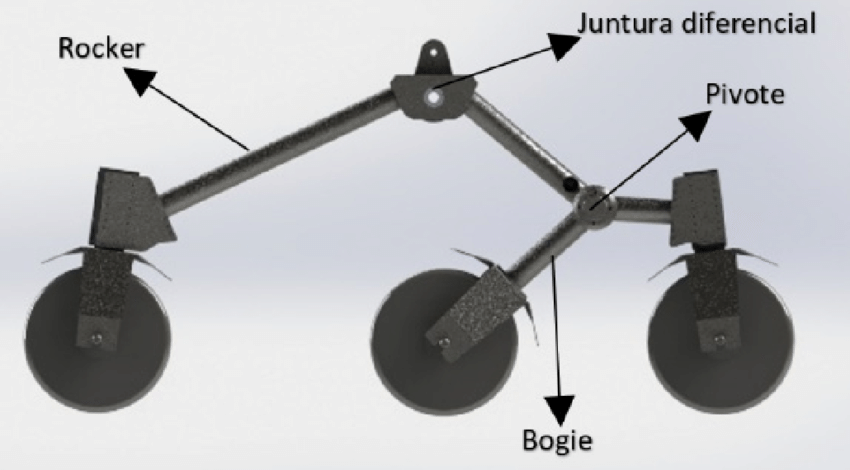
\includegraphics[width=\linewidth,height=3.4cm]{fig/rb-suspension.png}
  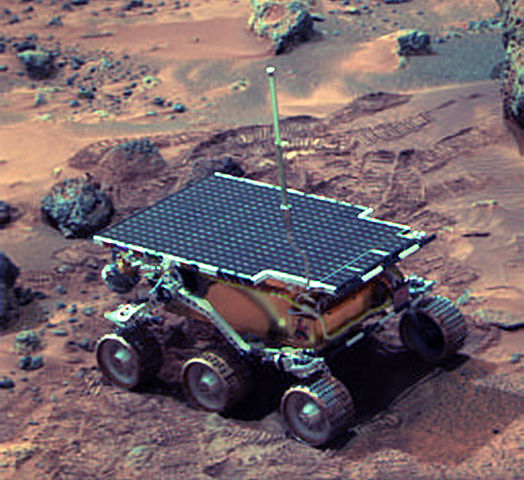
\includegraphics[width=.49\linewidth,height=3cm]{fig/sojourner.jpg}
  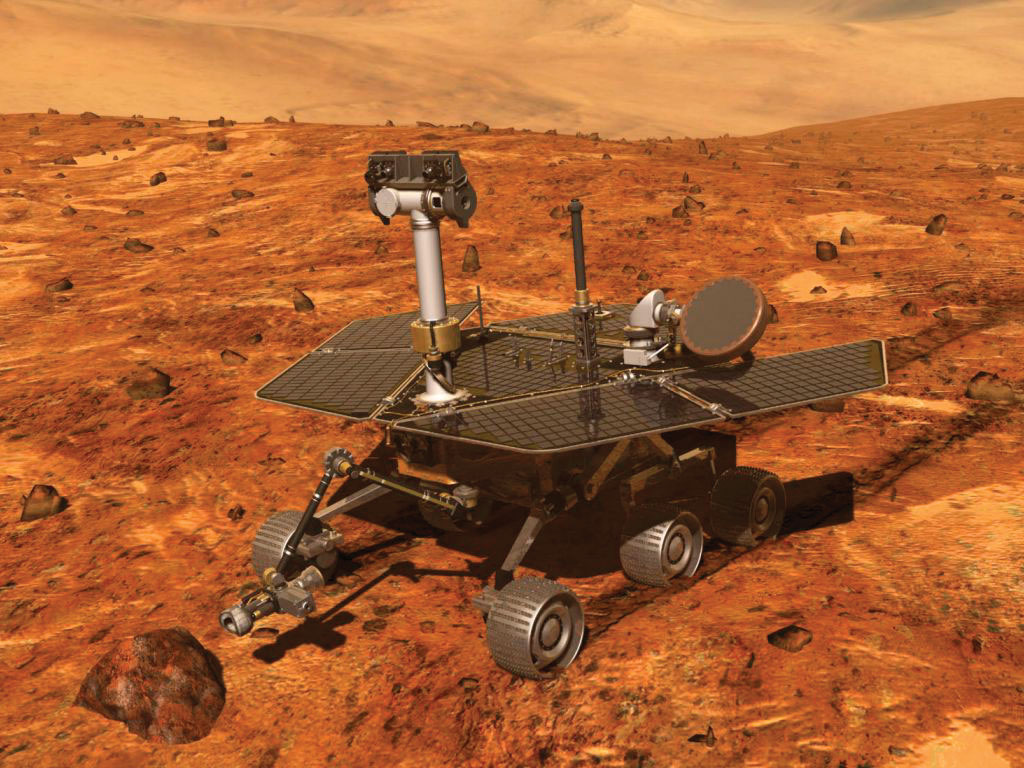
\includegraphics[width=.49\linewidth,height=3cm,trim={6cm 0 0 0},clip]{fig/spirit.jpg}
  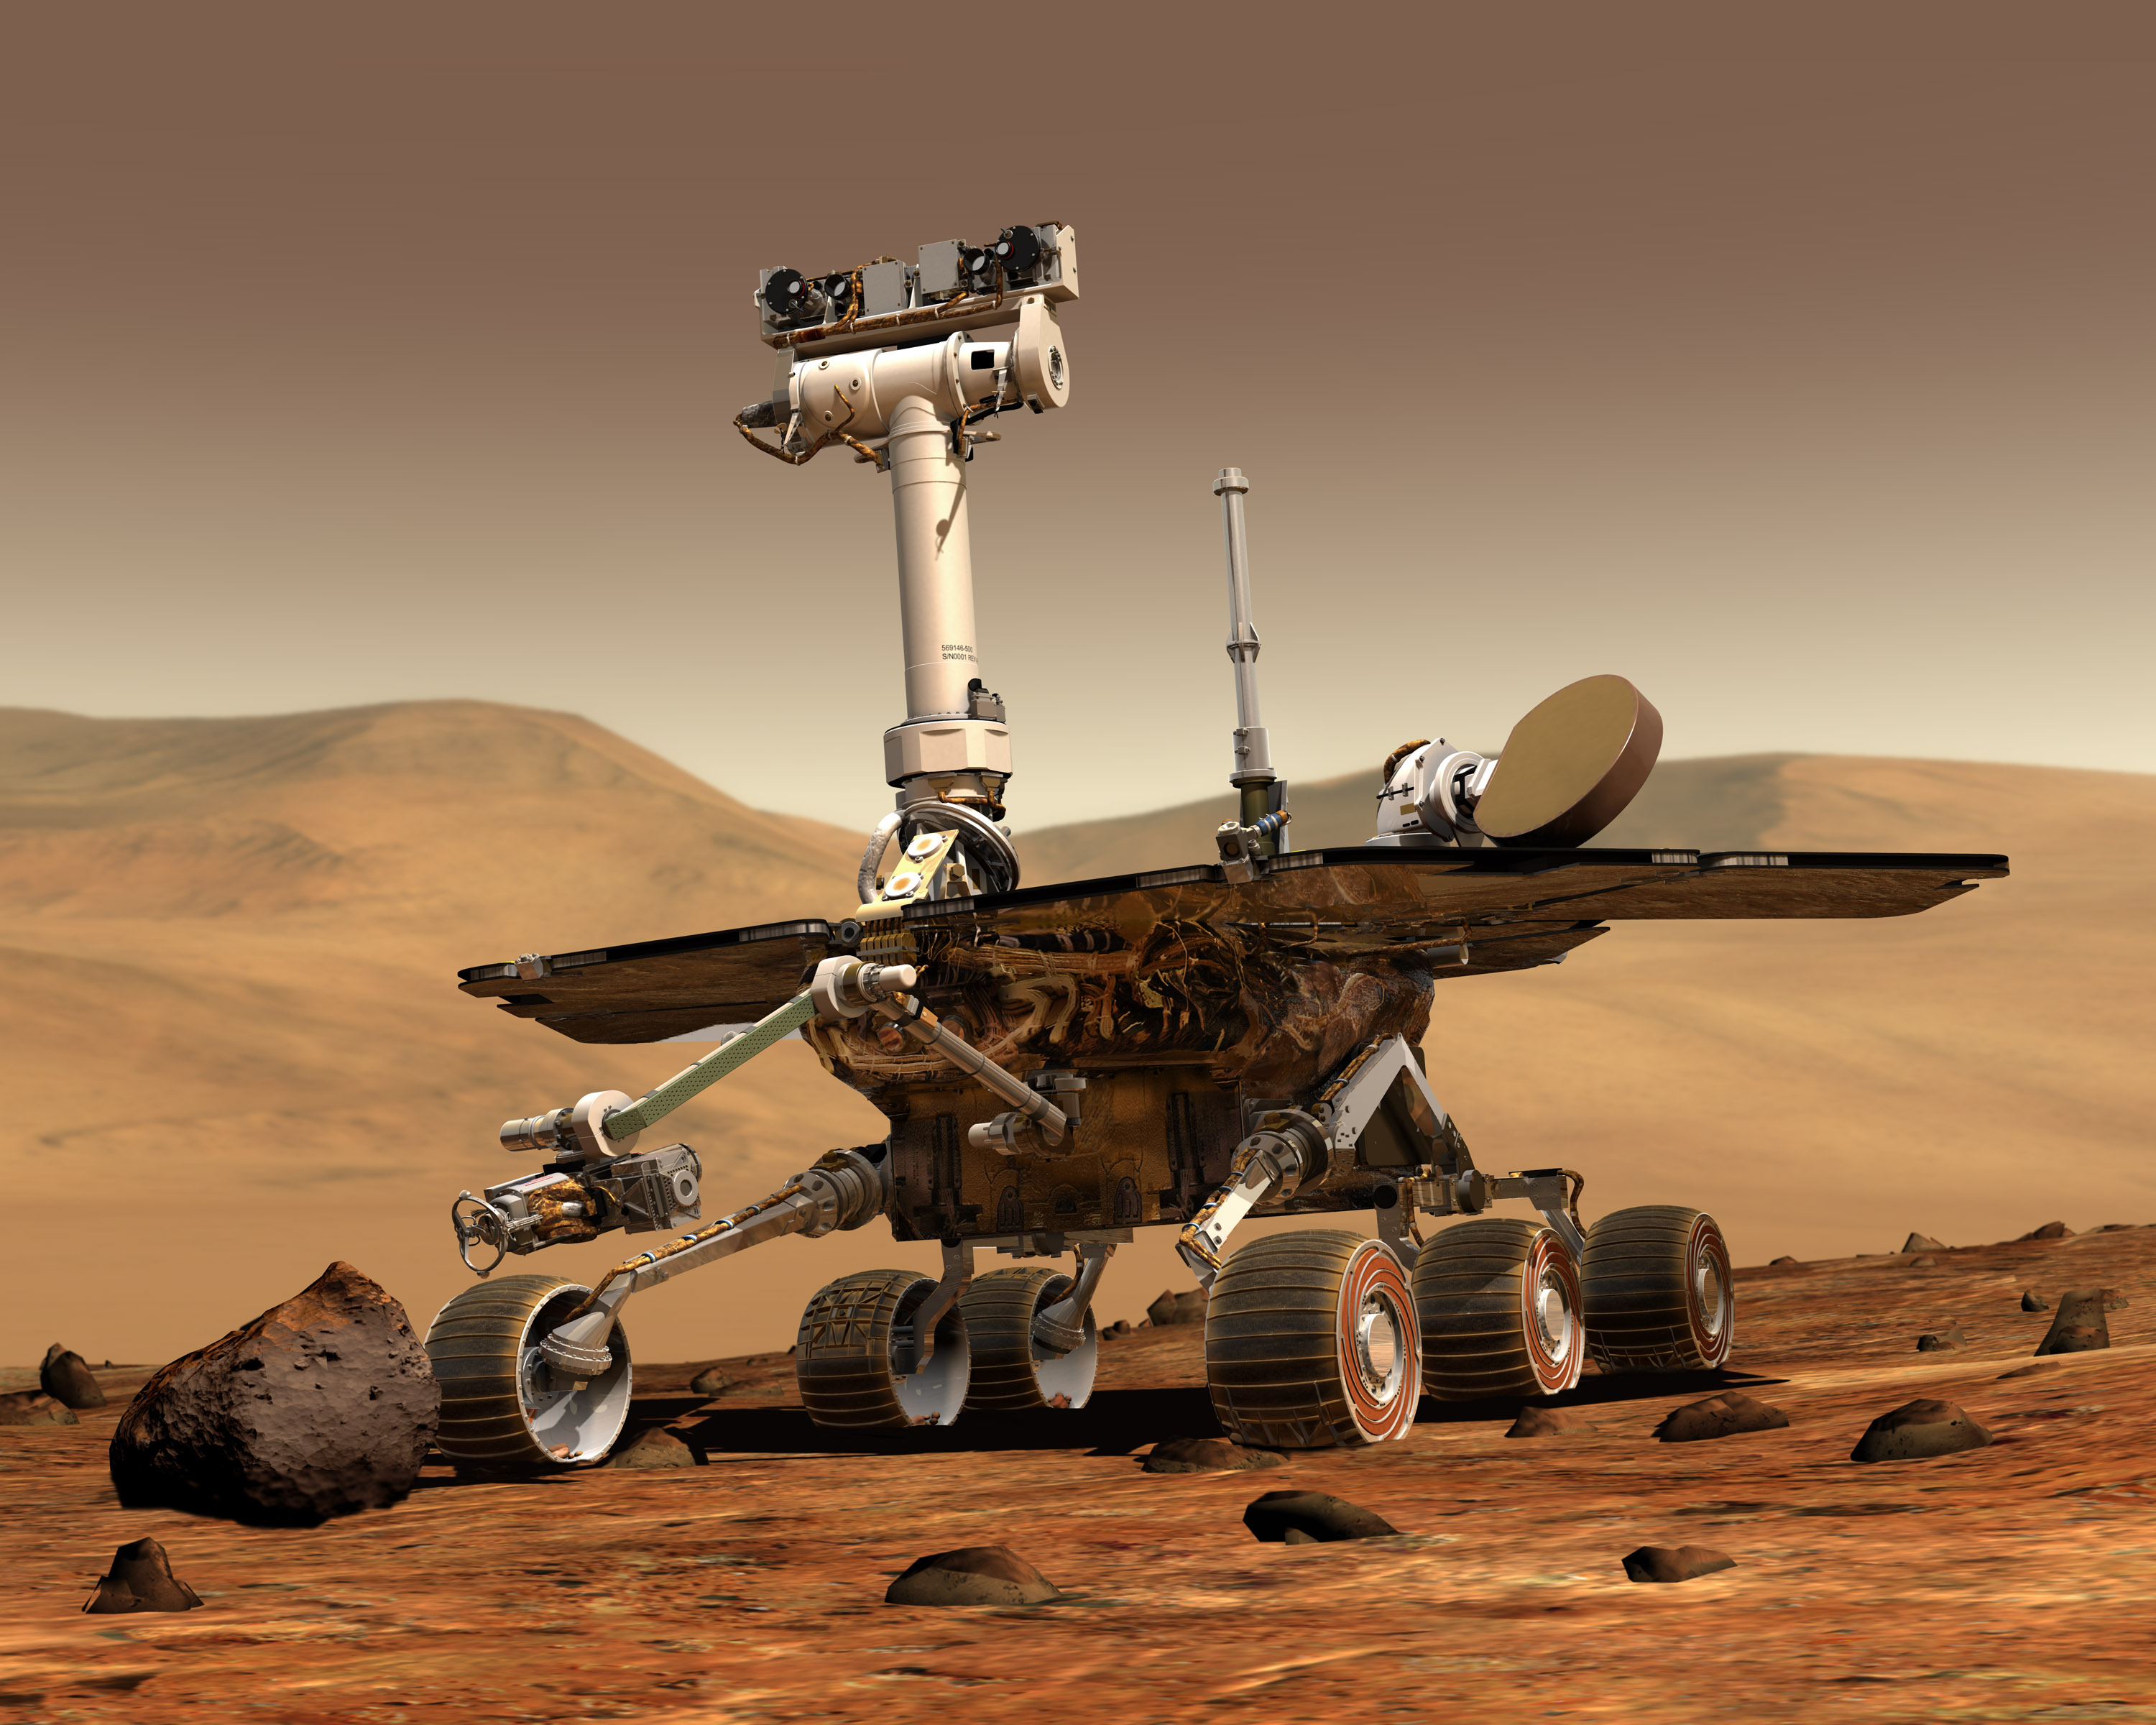
\includegraphics[width=.49\linewidth,height=3cm]{fig/opportunity.jpg}
  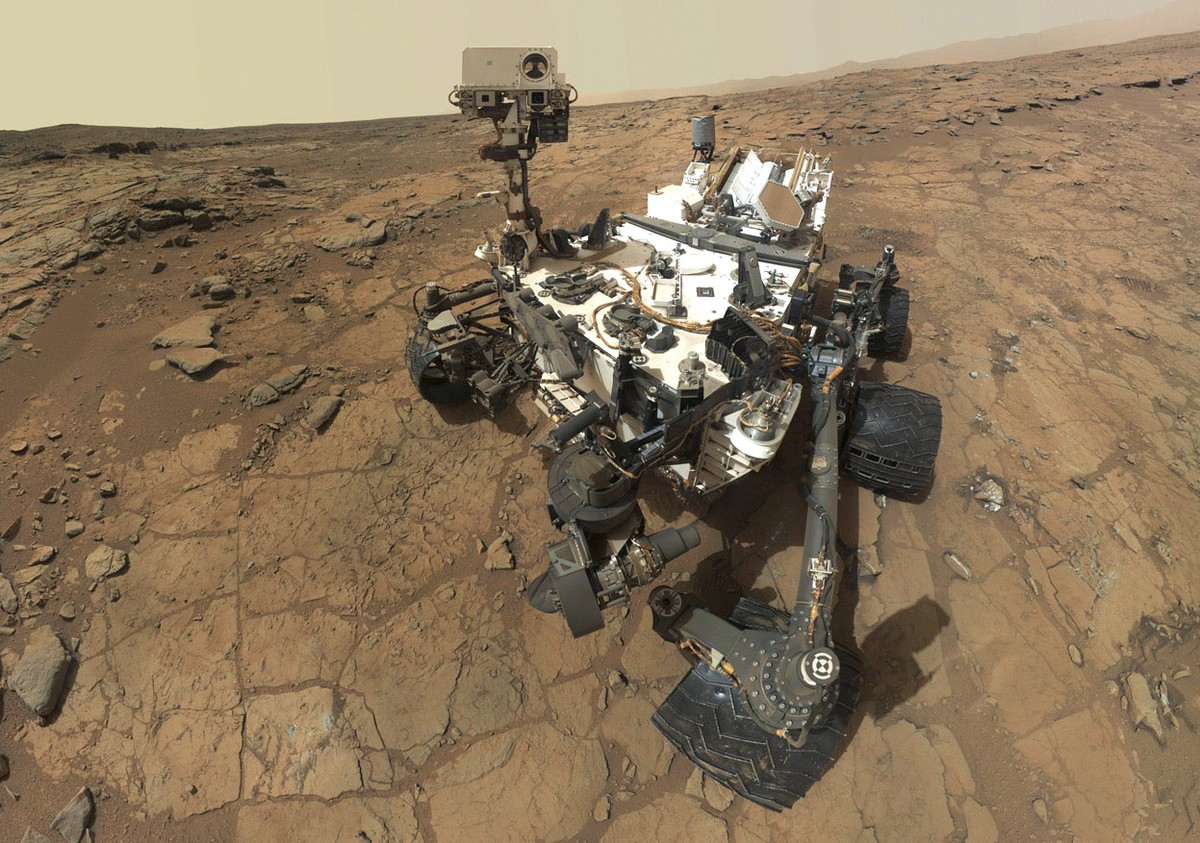
\includegraphics[width=.49\linewidth,height=3cm,trim={12cm 0 7cm 0},clip]{fig/curiosity.jpg}
  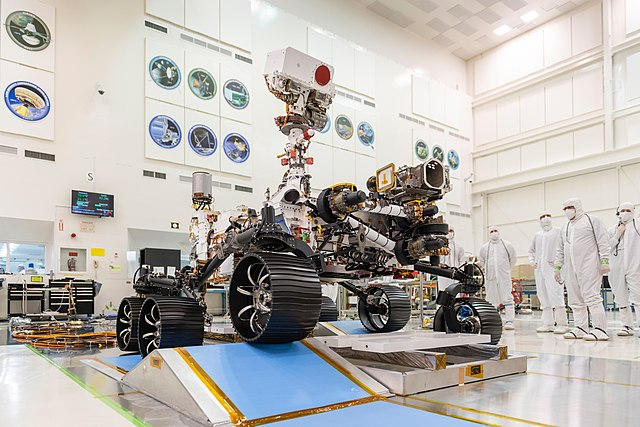
\includegraphics[width=\linewidth,height=3.5cm,trim={0 2.7cm 0 1.5cm},clip]{fig/perseverance.jpg}
  \captionof{figure}{Sistema rocker-bogie, Sojourner (1996), Spirit (2003), Opportunity (2003), Curiosity (2011) e Perseverance (2020).}
  \label{fig:int-1}
\end{minipage}

\pagebreak

O meu trabalho é sobre o sistema de suspensão rocker-bogie. Eu fiz este diagrama abaixo, mas tem algo errado com as equações.

\hspace{4cm}

\begin{figure}[h!]
  \begin{tikzpicture}
  \begin{scope}
    \point{a}{0}{0};
    \point{b}{5}{0};
    \point{c}{10}{0};
    \point{d}{7.5}{2.5};
    \point{e}{5}{5};

    \beam{2}{a}{e};
    \beam{2}{e}{c};
    \beam{2}{d}{b};

    \support{1}{a};
    \support{1}{b};
    \support{1}{c};

    \dimensioning{1}{a}{b}{-2}[L/2];
    \dimensioning{1}{b}{d}{-2}[L/4];
    \dimensioning{1}{d}{c}{-2}[L/4];
    \dimensioning{2}{d}{e}{11.5}[h/2];
    \dimensioning{2}{c}{d}{11.5}[h/2];

    \load{1}{e}[90];

    \dnotation{1}{e}{P}[yshift=9mm,right=1mm];
    \dnotation{1}{a}{A}[above left];
    \dnotation{1}{b}{B}[above left];
    \dnotation{1}{c}{C}[above right];
    \dnotation{1}{d}{D}[above right];
    \dnotation{1}{e}{E}[below=2mm];

    % \internalforces{a}{e}{0}{1};
  \end{scope}

  \begin{scope}[fill=blue]
    \internalforces{a}{e}{0}{1};
    \internalforces{b}{d}{0}{1};
    \internalforces{c}{d}{0}{1};
    \internalforces{d}{e}{0}{1};
  \end{scope}
\end{tikzpicture}
\end{figure}

\begin{align*}
  \sum F_H = 0 \;&\Rightarrow\; H_A + H_B + H_C = 0\\
  \sum F_V = 0 \;&\Rightarrow\; V_A + V_B + V_C - P = 0\\
  \sum M^{(A)} = 0 \;&\Rightarrow\; \frac{L}{2}V_A + LV_C - \frac{LP}{2} = 0\\
  \sum M^{(B)} = 0 \;&\Rightarrow\; \frac{-L}{2}V_A + \frac{L}{2}V_C = 0\\
  \sum M^{(C)} = 0 \;&\Rightarrow\; -LV_A - \frac{-L}{2}V_B + \frac{LP}{2} = 0\\
\end{align*}

\begin{figure}[h!]
  \centering
  \begin{minipage}{.5\textwidth}
    \begin{tikzpicture}
  \begin{scope}
    \point{a}{0}{0};
    \point{e}{2.5}{2.5};

    \beam{2}{a}{e};

    \support{1}{a};

    \hinge{1}{e};

    \load{1}{e}[90];

    \dnotation{1}{e}{P}[yshift=9mm,right=1mm];
    \dnotation{1}{a}{A}[above left];
    \dnotation{1}{e}{E}[below=2mm];

    \load{3}{e}[315][90][.8];
    \draw[->,thick] (e) -- (3.5,3.5);
    \draw[->,thick] (e) -- (3.5,1.5);

    \dnotation{1}{e}{$M_E$}[right=9mm];
    
  \end{scope}

  
\end{tikzpicture}
    \hfill
  \end{minipage}%
  \begin{minipage}{.5\textwidth}
    \hfill
    \begin{tikzpicture}
  \begin{scope}
    \point{c}{2.5}{0};
    \point{d}{0}{2.5};

    \beam{2}{c}{d};

    \support{1}{c};

    \hinge{1}{d};

    \dnotation{1}{c}{C}[above right];
    \dnotation{1}{d}{D}[above right];

    \draw[->,thick] (d) -- (-1,3.5);
    \draw[->,thick] (d) -- (-1,1.5);
    \load{2}{d}[135][90][.8]

    \dnotation{1}{d}{$M_D$}[left=9mm];
  \end{scope}
\end{tikzpicture}
  \end{minipage}
\end{figure}

Considerando os pontos D e E como articulações, eu consigo essas novas equações (que eu acho que estão erradas).

\begin{align*}
  \sum M^{(D)} = 0 \;&\Rightarrow\; \frac{L}{4}V_C + \frac{y}{2}H_C + \underbrace{M_D}_{0} = 0\\
  \sum M^{(E)} = 0 \;&\Rightarrow\; \frac{-L}{2}V_A + yH_A + \underbrace{M_E}_{0} = 0
\end{align*}

O sistema formado por essas seis equações não gera o número de equações LI suficientes para 
determinar os valores das 6 incógnitas, por isso acredito que as equações que escrevi estão erradas.
Gostaria de saber o que estou fazendo errado ou se existe uma forma melhor de fazer isso. 
Não sei se é melhor aplicar o método do equilíbrio dos nós.

\begin{empheq}[left=\empheqlbrace]{align}
  &\sum F_H = 0 \;\;\Rightarrow\;\; H_A + H_B + H_C = 0\\
  &\sum F_V = 0 \;\;\Rightarrow\;\; V_A + V_B + V_C - P = 0\\
  &\sum M^{(A)} = 0 \;\;\Rightarrow\;\; \frac{L}{2}V_A + LV_C - \frac{L}{2}P = 0\\
  &\sum M^{(B)} = 0 \;\;\Rightarrow\;\; -\frac{L}{2}V_A + \frac{L}{2}V_C = 0\\
  &\sum M^{(C)} = 0 \;\;\Rightarrow\;\; -LV_A - \frac{L}{2}V_B + \frac{L}{2}P = 0
\end{empheq}

\end{document}